\documentclass[11pt]{article}
\usepackage[a4paper,margin=2.2cm]{geometry}
\usepackage{amsmath}
\usepackage{graphicx}
\usepackage{booktabs}
\usepackage{parskip}
\usepackage{caption}

\setlength{\parindent}{0pt}
\pagestyle{empty}

\begin{document}

{\Large\bfseries C51 on Pong (object-centric): MLP width comparison}\\[2pt]
Group 27 \textbullet{} Topic 27 \textbullet{} JAXAtari baselines

\vspace{6pt}\hrule\vspace{8pt}

Three OC MLP widths, everything else held fixed (normalization, 10M frames, 8 envs,
identical hyperparameters). Final episodic return at 10M frames:

\vspace{4pt}
\begin{center}
\begin{tabular}{@{}lccl@{}}
\toprule
OC network & Layers & Final return (10M) & Status at 10M \\
\midrule
$512\times512$   & 2 & $\mathbf{+18.0}$ & solved, plateaued \\
$128\to64\to32$  & 3 & $\mathbf{+12.4}$ & solved late, still rising \\
$64\to32\to16$   & 3 & $\mathbf{-2.4}$  & mostly flat, steep unfinished climb \\
\bottomrule
\end{tabular}
\end{center}

\begin{figure}[h]
\centering
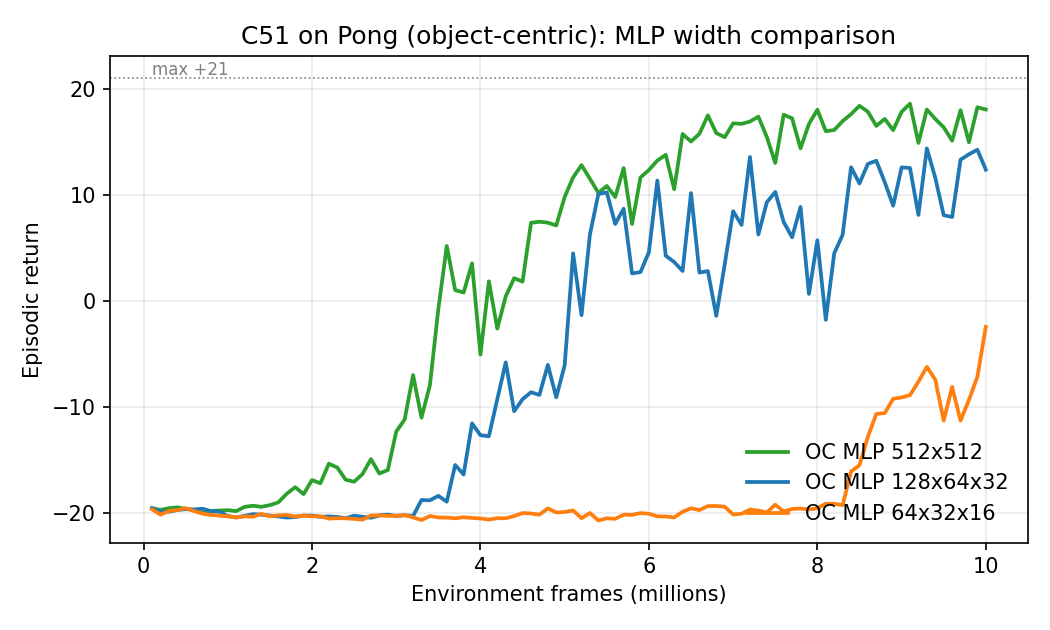
\includegraphics[width=0.82\linewidth]{c51_oc_width3_comparison.png}
\end{figure}

\textbf{Decision}
\begin{itemize}\itemsep0pt
  \item Stick with $\mathbf{512\times512}$: fastest and highest within 10M, only choice that plateaus.
  \item $128\to64\to32$ is a reasonable middle ground but leaves return on the table at 10M.
\end{itemize}

\end{document}
